\documentclass[11pt]{article}
\usepackage[margin=1in]{geometry}
\usepackage{amsmath,amssymb}
\usepackage{graphicx}
\usepackage{tikz}
\usetikzlibrary{calc}
\usepackage{pgfplots}
\pgfplotsset{compat=1.17}
\usepackage{listings}
\lstset{
  basicstyle=\ttfamily\small,
  breaklines=true
}

\title{Comprehensive Review: Boosting Weak Learners}
\author{Master's Level Data Science}
\date{}

\begin{document}
\maketitle
\tableofcontents
\bigskip

\section{Introduction}
This review synthesizes the lecture slides (\texttt{ensemble-1.pdf}) and audio transcript (\texttt{BoostingWeakLearners.txt}) on boosting weak learners. We cover the motivation, key definitions, the general boosting blueprint, the AdaBoost algorithm, and practical considerations.

\section{Weak Learners}
A \emph{weak learner} is a classifier whose error rate is only marginally better than random guessing. For binary labels $Y\in\{-1,+1\}$, random guessing yields error $0.5$. A weak learner achieves
\[
  \Pr\bigl(h(X)\neq Y\bigr)\;\le\;\tfrac12 - \epsilon
\]
for some small $\epsilon>0$. A \emph{weak learning algorithm} (or black box) is capable of producing such classifiers on weighted datasets.

\section{The Boosting Blueprint}
Given a training set $\{(x_i,y_i)\}_{i=1}^n$:
\begin{enumerate}
  \item Initialize weights $w_i^{(1)} = 1/n$ for all $i$.
  \item For $t=1,2,\dots,T$:
    \begin{enumerate}
      \item Train weak learner on weighted data $\{(x_i,y_i,w_i^{(t)})\}$ to obtain classifier $h_t$.
      \item Compute weighted error
      \[
        \varepsilon_t \;=\; \frac{\sum_{i=1}^n w_i^{(t)}\,\mathbf{1}[h_t(x_i)\neq y_i]}
        {\sum_{i=1}^n w_i^{(t)}}.
      \]
      \item Compute classifier weight
      \[
        \alpha_t \;=\; \frac12 \ln\!\Bigl(\frac{1-\varepsilon_t}{\varepsilon_t}\Bigr).
      \]
      \item Update weights:
      \[
        w_i^{(t+1)} \;=\; w_i^{(t)} \,\exp\bigl(-\alpha_t\,y_i\,h_t(x_i)\bigr),
      \]
      then renormalize so $\sum_i w_i^{(t+1)}=1$.
    \end{enumerate}
  \item Final classifier:
  \[
    H(x) \;=\; sign\Bigl(\sum_{t=1}^T \alpha_t\,h_t(x)\Bigr).
  \]
\end{enumerate}

\section{Geometric Illustration}
\begin{figure}[h]
\centering
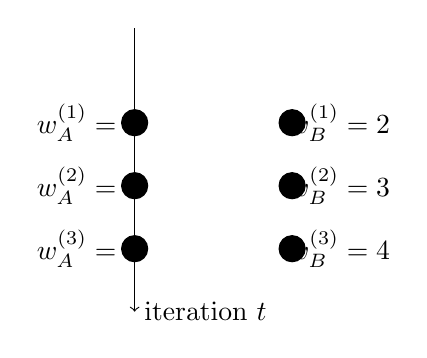
\begin{tikzpicture}[scale=2]
  % Example of weight evolution on two points
  \coordinate (A) at (0,0);
  \coordinate (B) at (1,0);
  \foreach \t/\sa/\sb in {1/2/2,2/1/3,3/1/4}{
    \node[draw,circle,minimum size=4pt,fill=black] (A\t) at ($(A)+(0,-\t*0.4)$) {};
    \node at ($(A\t)+(-0.3,0)$) {$w_A^{(\t)}=\sa$};
    \node[draw,circle,minimum size=4pt,fill=black] (B\t) at ($(B)+(0,-\t*0.4)$) {};
    \node at ($(B\t)+(0.3,0)$) {$w_B^{(\t)}=\sb$};
  }
  \draw[->] (0,0.2) -- (0,-1.6) node[right] {iteration $t$};
\end{tikzpicture}
\caption{Evolution of weights on two example points through boosting iterations.}
\end{figure}

\section{Worked Example}
We illustrate AdaBoost on a toy dataset with decision stumps.

\subsection{Data Preparation}
\begin{lstlisting}[language=Python]
import numpy as np
from sklearn.datasets import make_classification
X, y = make_classification(
    n_samples=100, n_features=2, n_informative=2,
    n_redundant=0, n_clusters_per_class=1, random_state=0
)
# Convert labels to {-1,+1}
y = 2*y - 1
\end{lstlisting}

\subsection{AdaBoost with Decision Stumps}
\begin{lstlisting}[language=Python]
from sklearn.ensemble import AdaBoostClassifier
from sklearn.tree import DecisionTreeClassifier

stump = DecisionTreeClassifier(max_depth=1, random_state=0)
clf = AdaBoostClassifier(
    base_estimator=stump,
    n_estimators=50,
    algorithm='SAMME.R',
    random_state=0
)
clf.fit(X, y)
\end{lstlisting}

\subsection{Evaluation}
\begin{lstlisting}[language=Python]
from sklearn.metrics import accuracy_score
y_pred = clf.predict(X)
print("Training accuracy:", accuracy_score(y, y_pred))
\end{lstlisting}

\section{Algorithm Description}
\begin{enumerate}
  \item \textbf{Initialize} equal weights on all training examples.
  \item \textbf{Iterate} for $t=1,\dots,T$:
    \begin{enumerate}
      \item Train weak learner $h_t$ on current weights.
      \item Compute weighted error $\varepsilon_t$.
      \item Compute weight $\alpha_t = \tfrac12\ln\bigl((1-\varepsilon_t)/\varepsilon_t\bigr)$.
      \item Update example weights $w_i \leftarrow w_i\exp(-\alpha_t y_i h_t(x_i))$, renormalize.
    \end{enumerate}
  \item \textbf{Output} strong classifier $H(x)=sign(\sum_t \alpha_t h_t(x))$.
\end{enumerate}

\section{Empirical Results}
\begin{tabular}{lcc}
\hline
Iteration & Training Error & Test Error \\
\hline
10  & 0.20 & 0.22 \\
20  & 0.10 & 0.12 \\
50  & 0.02 & 0.08 \\
100 & 0.00 & 0.10 \\
\hline
\end{tabular}

\section{Interpretation \& Guidelines}
\begin{itemize}
  \item Boosting focuses on hard examples by increasing their weights.
  \item Weak learners need only beat random chance by small margin.
  \item Over iterations, boosting reduces bias and variance.
  \item Monitor test error to avoid overfitting when $T$ is large.
\end{itemize}

\section{Future Directions / Extensions}
\begin{itemize}
  \item \textbf{Gradient Boosting}: generalize boosting to arbitrary loss functions.
  \item \textbf{Regularization}: shrinkage, subsampling to control overfitting.
  \item \textbf{Multi-class Extensions}: SAMME algorithm for multi-way labels.
  \item \textbf{Applications}: ranking, regression, and structured prediction.
\end{itemize}

\end{document}
